\documentclass[12pt,a4paper]{article}
\usepackage[T1]{fontenc}
\usepackage[utf8]{inputenc}
\usepackage[margin=2.5cm]{geometry}
\usepackage[francais]{babel}
\usepackage{graphicx}


\begin{document}
\title{Projet A.L.A.M.\\ Systèmes de recommandation DIY}
\date{\today}
\author{Louis Becquey - 3BIM}
\maketitle
\newpage

\section{Question A - Chargez les données}
Les données du site movielens.org sont chargées dans des dictionnaires python.
\section{Question B - Matrice Utilisateur-Item}
On construit une matrice R de 943 lignes (les utilisateurs) et 1682 colonnes (les films).
\begin{figure}[h!]
	\centering
	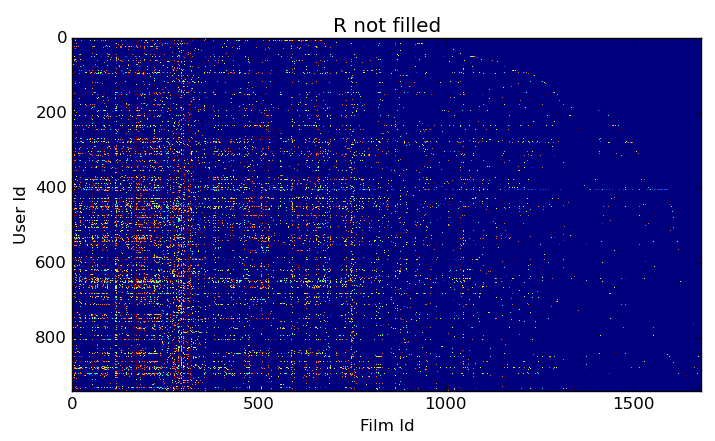
\includegraphics[scale=0.5]{R-Not-Filled.png}
	\caption{Matrice $R$ de données: Bleu=Pas de vote, couleurs du vert au rouge=note de 1 à 5 étoiles.}
\end{figure}
\\
On remarque qu'il existe des films qui n'ont été notés par personne, cependant, il n'existe pas d'utilisateur qui n'aie voté pour aucun film.
\newpage

\section{Question C - Approximation bas-rang par SVD}
On remplit les données manquantes de la matrice $R$ de deux façons différentes, en utilisant la moyenne des notes de ce film, ou en utilisant la moyenne des notes de cet utilisateur.\\

\begin{figure}[h!]
	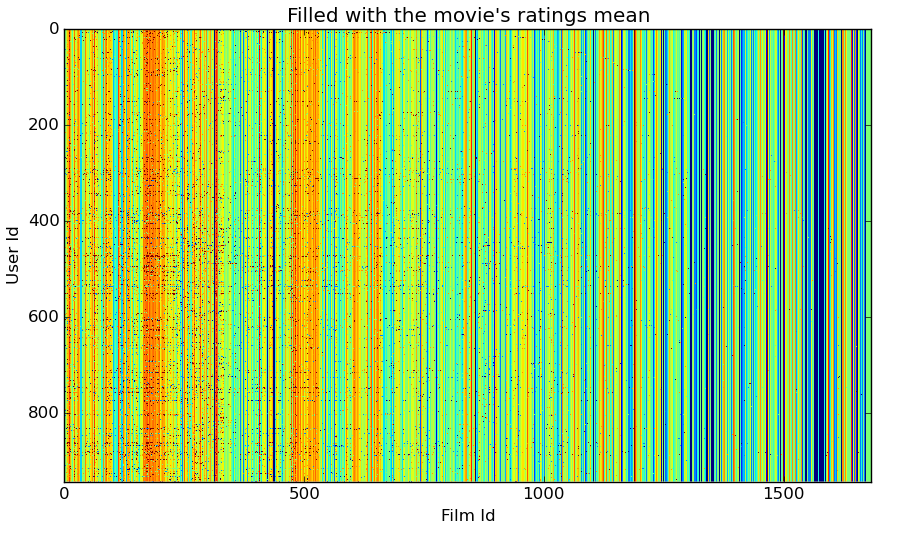
\includegraphics[scale=0.28]{R-Filled-By-Movie.png}
	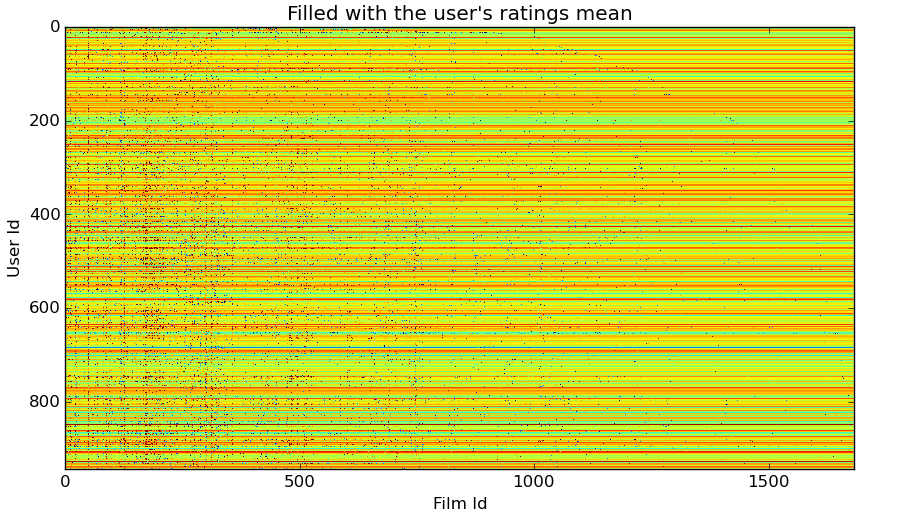
\includegraphics[scale=0.28]{R-Filled-By-User.png}
	\caption{A droite: Matrice $Rc$ remplie avec la moyenne du film lors de données manquantes. A gauche: Matrice $Rr$ remplie avec la moyenne de l'utilisateur lors de données manquantes.}
\end{figure}

On utilisera \texttt{ numpy.linalg.svd() } pour calculer les décompositions en valeurs singulières. $$R=USV'$$On réalise ensuite l'approximation de $Rc$ ou $Rr$ en ne retenant que $k$ valeurs singulières sur $m$.\\ Éliminer les $(m-k)$ dernières valeurs singulières revient à éliminer dans le calcul les valeurs des $(m-k)$ dernières colonnes de $U$ et des $(m-k)$ dernières lignes de $V'$.\\
Donc à partir de $U$ de taille $m\times m$, $S$ de taille $m \times m$ et $V'$ de taille $m \times n$, on ne garde que $U_k$ une matrice de taille $m \times k$, $S_k$ de taille $k \times k$ et $V'_k$ de taille $k \times n$.
$$R \approx U_kS_kV'_k$$

$\Rightarrow$ Comprendre Xk et Yk, et Xk(u,) et Yk(:,i)

\newpage
\section{Question D - Qualité de la prédiction par SVD}
On peut estimer l'erreur par la moyenne (en note) des différences entre la note réelle dans l'échantillon test et celle prévue par l'approximation de rang k (en valeur absolue), dite MAE (Mean Absolute Error).\\

\begin{figure}[h!]
	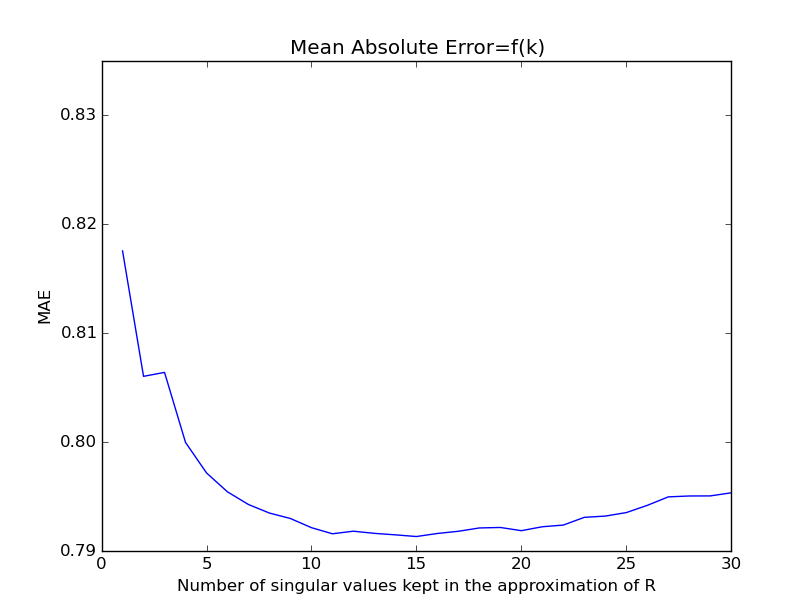
\includegraphics[scale=0.38]{MAE-By-Movie.png}
	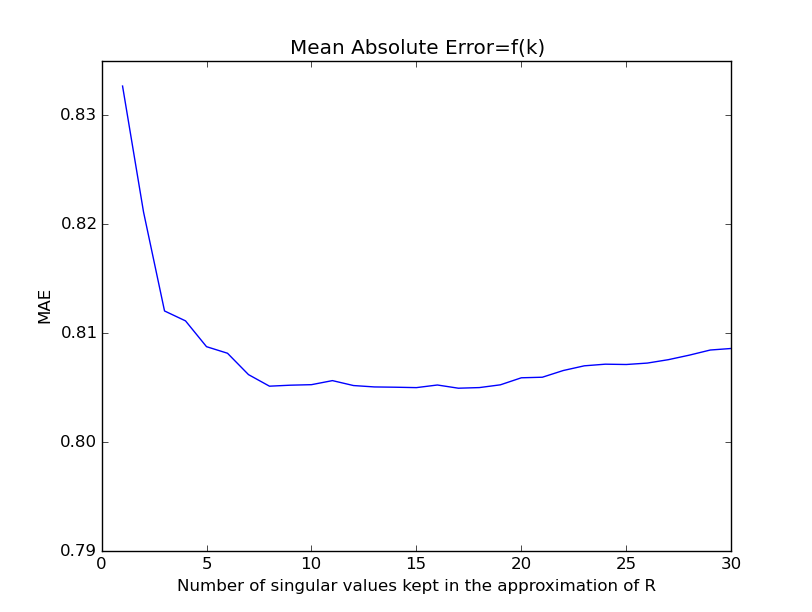
\includegraphics[scale=0.38]{MAE-By-User.png}
	\caption{A droite: MAE selon le rang de l'approximation, pour Rc (moyenne du film) à gauche, et pour Rr (moyenne de l'utilisateur) à droite.}
\end{figure}

On remarque donc que la méthode naïve utilisant la moyenne du film est légèrement plus fidèle.\\
En prenant k=12, on arrive à se limiter à une erreur d'environ 0,792 par note.\\
Il est important de se rappeler que cette note est attribuée en étoiles de 1 à 5, sans décimales. On pourrait donc arrondir l'erreur et considérer que cette méthode est précise à plus ou moins 1 étoile.\\

Si ensuite on souhaite mesurer l'erreur due à l'approximation par SVD, on peut là aussi faire la moyenne des différences (en valeur absolue) entre la matrice remplie par méthode naïve et l'approximation de cette même matrice, avec k=12.\\
On obtient, pour Rr comme pour Rc, une erreur d'environ 0,06 étoile, ce qui est faible et tout à fait satisfaisant.\\

En effet, l'approximation de la matrice permet d'\textbf{économiser énormément d'espace de stockage} (dans notre exemple: $943\times1682=1586126$ contre $943\times12+1682\times12+12\times12=31644$ soit un facteur 50). En revanche, le \textbf{temps de calcul est plus long} puisque l'on doit calculer deux produits pour obtenir le résultat. Et ceci pour une \textbf{différence de qualité de précision faible} étant donné la MAE de la méthode en général face aux réelles valeurs de l'échantillon test (0,06 contre 0,79).

\section{Question E - Théorie}
Montrons que si une matrice A est réelle, alors elle admet une décomposition en valeurs singulières $A=U \Sigma V^{*}$, avec U et V des matrices à coefficients réels.

$\Rightarrow$ Euh...

\section{Question F - Problème des moindres carrés pour méthode alternée}
On a pour objectif d'obtenir $X.Y\approx R$. Le rôle de la ligne $X_u$ dans ce produit est de permettre de calculer les valeurs de la ligne $R_u$ dans la matrice finale. Ainsi, 
$$X_u.Y\approx R_u$$
$$(X_u.Y)^T\approx (R_u)^T$$
$$Y^T.X_u^T\approx R_u^T$$
où $Y^T$ est une matrice $n\times k$, et $X_u^T$ et $R_u^T$ deux vecteurs colonnes, $R_u^T$ connu. \\
Il s'agit donc d'un problème des moindres carrés linéaire.\\

Et plus directement, le rôle de la colonne $Y_i$ est de permettre le calcul des valeurs de la colonne $R_i$, donc:
$$X.Y_i \approx R_i$$
Il s'agit là aussi d'un problème des moindres carrés linéaire.



\end{document}